\chapter{Konzept}
\label{konzept}

% Wie funktionieren die Tests, ganz grob?
Um die drei Algorithmen zu vergleichen,
	werden verschiedene Tests durchgeführt.
Diese speisen verschiedene Lieder eines Testdatensatzes in die jeweiligen Algorithmen ein
	und nehmen dabei deren Ausgabe auf.
Aus diesen Testaufzeichnungen werden Metriken berechnet,
	die es ermöglichen,
	die Algorithmen miteinander zu vergleichen.

% Kapitelübersicht
In Abschnitt~\ref{konzept/ziele} wird erklärt,
	was die Ziele der einzelnen Tests sind
	und welche Fragen durch die Tests beantwortet werden sollen.
In Abschnitt~\ref{konzept/testdaten} wird der verwendete Datensatz vorgestellt
	und in Abschnitt~\ref{konzept/gestaltung} wird die Umsetzung der Tests beschrieben.


\section{Ziele} \label{konzept/ziele}
{
	Bevor man sinnvolle Vergleichstests konzipieren kann,
		muss zuerst festgestellt werden,
		unter welchen Gesichtspunkten die Algorithmen verglichen werden können.

	% Tempo
	Alle drei Algorithmen geben eine Schätzung des Tempos des aktuellen Songs aus.
	Daraus ergibt sich follgende die erste Forschungsfrage.
	\begin{equation}
		\label{question:tempo}
		\text{\emph{Wie hoch ist die Genauigkeit der Temposchätzungen?}}
	\end{equation}

	% Beatzeitpunkte
	Au{\ss}erdem liefern die Algorithmen von~\cite{2009_DaPlSt} und~\cite{2011_PlRoSt} zusätzlich noch Informationen zur Position des aktuellen oder nächsten Beats.
	So gibt~\cite{2011_PlRoSt} beispielsweise die Phase aus,
		welche die Position des Beats innerhalb des aktuellen Beatintervalls angibt.
	Daraus lassen sich die absoluten Beatzeitpunkte berechnen.
	Da das System von~\cite{2009_DaPlSt} direkt absolute Beatzeitpunkte ausgibt,
		können diese als Grundlage für einen weiteren Vergleich der beiden Algorithmen verwendet werden.
	Dies wirft zwei weitere Forschungsfragen auf.
	\begin{align}
		\label{question:beat}
		\text{\emph{Wie hoch ist die Genauigkeit der Vorhersage der Beatzeitpunkte?}} \\
		\label{question:streak}
		\text{\emph{Wie lang ist die längste korrekt bestimmte Beatfolge?}}
	\end{align}

	% CPU-Zeit
	Alle Algorithmen nutzen CPU-Ressourcen.
	Folglich kann untersucht werden,
		welcher Algorithmus am effizientesten damit umgeht.
	Vor diesem Hintergrund reiht sich eine letzte Forschungsfrage ein.
	\begin{equation}
		\label{question:cpu_time}
		\text{\emph{Wie viel CPU-Zeit wird im Echtzeitbetrieb pro Sekunde benötigt?}}
	\end{equation}
}

\section{Testdaten} \label{konzept/testdaten}
{
	% allgemeines Gelaber
	Als Testdatensatz wurde der Datensatz von~\cite{2012_HoDaZaOlGo} verwendet,
		da es einer der wenigen Datensätze ist,
		der frei erhältlich ist
		und per Hand mit Beatzeitpunkten annotiert ist.
	Um die Leistungsfähigkeit von Beaterkennungsalgorithmen bestimmen zu können,
		ist es wichtig,
		einen manuell annotierten Datensatz zu verwenden.
	Wäre der Datensatz automatisch annotiert worden,
		würde man nur den eigenen Beaterkennungsalgorithmus mit dem,
		der für die Annotation verwendet wurde,
		vergleichen.

	% Woher kommen die Daten?
	Der verwendete Datensatz wurde aus Audio-CDs extrahiert.
	Folglich haben alle Dateien eine Abtastfrequenz von \SI{44.1}{\kilo\hertz}
		und es ist kein Resampling notwendig.
	Aus den CDs wurden von jedem Song \num{40} Sekunden extrahiert.
	% Art der Musik
	Die Auswahl der Lieder beschränkt sich ausschlie{\ss}lich auf westliche Musik.
	Dabei sind verschiedene Musikrichtungen vertreten,
		unter anderem: Klassik, Romantik, Filmmusik, Blues, Chanson und Sologitarrenkompositionen.
	% Wie groß?
	Der Datensatz besteht aus 217 Liedern.
	Davon haben 19 Lieder einen einfachen leicht erkennbaren Rhythmus.
	% Warum schwierige Rhythmen?
	Viele bisherige Datensätze enthalten Musik aus Rock-, Pop- oder Dance-Genres
		mit leicht erkennbaren Beats,
		die klar durch Schlagzeugtöne definiert sind.
	% TODO: 
	Dies erleichtert den Beaterkennungsalgorithmen,
		die korrekten Beatzeitpunkte zu finden.
	Da aktuelle Systeme auf den einfachen Datensätzen bereits fast perfekte Ergebnisse erzielen,
		bleibt somit kaum Spielraum für weitere Verbeserung.
	Um dem entgegenzuwirken,
		haben die Autoren dieses Datensatzes absichtlich schwierige Rhythmen ausgewählt.

	% Labels
	Zu jedem Exzerpt eines Liedes gibt es eine Annotationsdatei,
		welche die Liste der Beatzeitpunkte in diesem Lied enthält.
	Das Tempo des Liedes an einem bestimmten Zeitpunkt wird durch den Kehrwert des aktuellen Beatintervalls bestimmt.
}

\section{Gestaltung der Tests} \label{konzept/gestaltung}
{
	Die Testsoftware besteht aus zwei Komponenten:
		Datenakquisition und Datenauswertung.
	% TODO: hier vlt noch aweng rein, warum die beiden Komponenten getrennt sin

	\subsection{Datenakquisition}
	{
		% Was die Datenakquisition grob macht
		Die Datenakquisitionskomponente ruft die einzelnen Beaterkennungsalgorithmen auf
			und wurde in C++ implementiert
			um sie mit den Algorithmen zu linken.
		Es wird jedes Lied im Testdatensatz einmal in jeden der drei Algorithmen gegeben
			und dabei deren Ausgaben in einer CSV-Datei gespeichert.
		Dabei entsteht eine Datei pro Lied und Algorithmus.
		Die Algorithmen werden vor jedem Song neu initialisiert.

		% Was bei welchem Alg. aufgezeichnet wird und wie
		Bei~\cite{2001_BeatThis} wird nur jede neue Tempovorhersage aufgezeichnet.
		Bei~\cite{2009_DaPlSt} und~\cite{2011_PlRoSt} werden zusätzlich die vorhergesagten Beatzeitpunkte gespeichert.
		Die Tempovorhersagen von~\cite{2011_PlRoSt} werden nur dann gespeichert,
			wenn sie sich im Vergleich zur letzten Tempovorhersage geändert haben.
		Da der Algorithmus alle \SI{11.61}{\milli\second} eine neue Tempovorhersage ausgibt,
			ist das bei diesem Algorithmus notwendig,
			um die Grö{\ss}e der CSV-Dateien zu reduzieren.
		Da \cite{2011_PlRoSt} nicht direkt Beatzeitpunkte ausgibt,
			sondern eine Beatperiode $T$ und Phase $x$,
			welche ständig aktualisiert werden,
			wird anhand dieser Information der nächste Beatzeitpunkt berechnet
			und erst dann gespeichert,
			wenn er erreicht wird.
		Somit wird sichergestellt,
			dass jede Beatvorhersage nur einmal in der CSV-Datei auftritt.
		Gibt es ein $k \in \mathbb{N}$, das die Gleichung $kT + x = t$ erfüllt,
			wobei $t$ der aktuelle Zeitpunkt ist,
			dann wird $t$ als Beatzeitpunkt gespeichert.

		% CPU-Zeit-Messung
		Die API der Beaterkennungsalgorithmen funktioniert so,
			dass jedes Audiosample separat und nacheinander per Funktionsaufruf in das System gegeben wird.
		Alle Berechnungen laufen in Subroutinen dieser Funktion ab.
		Um die Gesamtrechenzeit des Algorithmus zu bestimmen,
			wird die CPU-Zeit von jedem dieser Funktionsaufrufe gemessen und aufsummiert.
	}

	\subsection{Datenauswertung}
	{
		% allgemeines Gelaber
		In der Datenauswertungskomponente der Testsoftware,
			werden lediglich die gepseicherten CSV-Dateien verarbeitet.
		So konnte diese unabhängig von der Implementierung der Algorithmen und deren Programmiersprache programmiert werden.
		Hier entsehen vier Auswertungen,
			welche sich auf die vier Fragen aus Anschnitt~\ref{konzept/ziele} beziehen.

		\paragraph{Tempofehler}
		{
			% Wie Tempofehler berechnet werden
			Um die Genauigkeit der Temposchätzungen zu bestimmen,
				wird ein Fehlerhistogram der Temposchätzungen erstellt.
			Dazu muss erst für jeden Algorithmus eine Liste aller Fehler her.
			Da die einzelnen Algorithmen ihre Temposchätzungen in unterschiedlichen Abständen aktualisieren
				(bzw. bei~\cite{2011_PlRoSt} nur wenn sich das Tempo ändert),
				wäre es unfair für jede Temposchätzung einen Fehler zu berechnen.
			Gibt~\cite{2011_PlRoSt} beispielswei{\ss}e ein konstant falsches Tempo über einen längeren Zeitraum aus,
				würde er nur einmal dafür bestraft werden,
				während einer der anderen beiden Algorithmen für jede einzelne falsche Temposchätzung in diesem Zeitraum bestraft werden würde.
			Aus diesem Grund wird ein Fehler für jedes Beatinterval berechnet.
			So enthalten am Ende alle drei Fehlerlisten gleich viele Fehler.
			Das korrekte Tempo wird aus dem Kehrwert des aktuellen Beatintervals berechnet,
				welches wiederum aus der Differenz des nächsten und des letzten Beatzeitpunktes bestimmt wird.
			Der Fehler des aktuellen Intervals ergibt sich aus der Differenz der aktuellen Tempovorhersage und dem korrekten Tempo.
			Alle Temposchätzungen vor dem ersten und nach dem letzten Beat werden ignoriert,
				da für diese Bereiche kein korrektes Tempo bestimmt werden kann.
			Gibt es im aktuellen Beatinterval keine Temposchätzung,
				wird die vorherige Schätzung genommen,
				bzw. dieses Interval übersprungen,
				wenn es bis zum aktuellen Zeitpunkt noch keine Schätzung gab.
			Gibt es mehrere Temposchätzungen,
				wird der Mittelwert genommen.

			% Halb- und Doppeltempofehler
			Weil das Problem der Tempobestimming nicht eindeutig ist,
				treten bei solchen Systemen häuft Halbtempo- und Doppeltempofehler auf.
			Das hei{\ss}t,
				der Algorithmus schätzt genau die Hälfte, bzw. das Doppelte, des richtigen Tempos.
			Liegt das korrekte Tempo au{\ss}erhalb des Wertebereichs,
				(\SIrange{80}{160}{BPM} bei allen Algorithmen in dieser Arbeit),
				ist die beste Ausgabe,
				die ein Algorithmus machen kann,
				zwangsläufig das halbe oder doppelte Tempo.
			Solche Fehler sind nicht schlimm
				und um sie zu berücksichtigen,
				wird für jedes Beatinterval nicht nur die Differenz zum korrekten Tempo,
				sondern auch die Differenz zum halben und zum doppelten Tempo berechnet.
			So entstehen pro Song pro Algorithmus drei Fehlerlisten.
			Die Liste mit der kleinsten Summe der Quadrate wird der Gesamtfehlerliste des Algorithmus angehängt.
			Die Gesamtfehlerliste kann anschlie{\ss}end als Histogram dargestellt werden.
		}

		\paragraph{Beatzeitpunktfehler und längste korrekte Beatfolge}
		{
			% Pairing
			Für die Bestimmung der Beatzeitpunktfehler,
				muss zunächst für jeden korrekten Schlag $C_n$ der dazugehörige Schlag in der Ausgabe des Algorithmus $B_n$ gefunden werden.
			Dafür wird der Ansatz des Pairings von~\cite{1997_GoMu1} verwendet.
			Es werden für jeden korrekten Beat $C_n$ alle ausgegebenen Beats $B_m$ gesucht,
				die die folgende Ungleichung erfüllen.
			\begin{equation}
				C_n - \frac{1}{2}(C_n - C_{n - 1}) \le B_m < C_n + \frac{1}{2}(C_{n + 1} - C_n)
			\end{equation}
			Gibt es kein $B_m$,
				welches die Ungleichung erfüllt,
				wird $C_n$ als ungepaar markiert.
			Falls es genau ein $B_m$ gibt,
				welches die Ungleichung erfüllt,
				wird ein Paar $(C_n, B_m)$ gebildet.
			Werden für ein $C_n$ mehrere mögliche $B_m$ gefunden,
				dann bildet $C_n$ ein Paar mit dem $B_m$,
				das den kleinsten Paarfehler (s. unten) erziehlt.
			Die anderen $B_m$ werden als ungepaart markiert.

			% Paarfehler
			Für jedes Paar $(C_n, B_m)$ wird ein normalisierter Fehler $P$ berechnet,
				der zwischen \num{0} und \num{1} liegt,
				wobei \num{0} bedeutet,
				dass $B_m$ genau auf dem korrekten Beat $C_n$ liegt,
				und \num{1},
				dass $B_m$ genau in der Mitte zwischen dem korrekten und dem nächsten oder vorherigen Beat liegt.
			\begin{equation}
				P((B_m, C_n)) =
					\begin{cases}
						\frac{2|B_m - C_n|}{C_{n + 1} - C_n} & \text{falls } B_m \ge C_n \vspace{3mm} \\
						\frac{2|B_m - C_n|}{C_n - C_{n - 1}} & \text{falls } B_m  <  C_n
					\end{cases}
			\end{equation}
			Alle ungepaarten Beats,
				sowohl aus $C_n$ als auch aus $B_n$ erhalten einen Fehler von \num{1}.

			\begin{figure}[h]
				\centering
				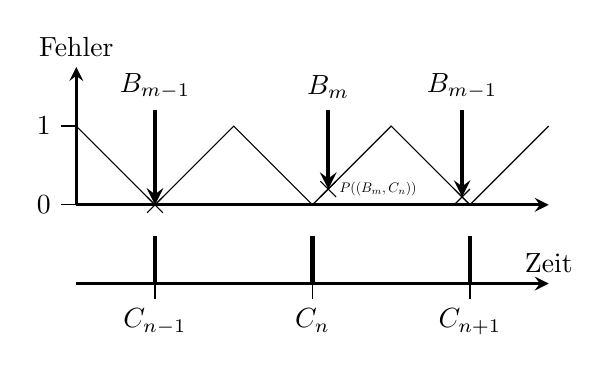
\begin{tikzpicture}
					\tikzstyle{axis} = [very thick, ->, >=stealth]
					\tikzstyle{tick} = [thin];
					\tikzstyle{cbeat} = [ultra thick]
					\tikzstyle{bbeat} = [ultra thick, ->, >=stealth]
					\tikzstyle{graph} = []

					\draw [axis] (0, -1) -- (6, -1) node [anchor=south] {Zeit};
					\draw [axis] (0, 0) -- (6, 0);
					\draw [axis] (0, 0) -- (0, 1.75) node [anchor=south] {Fehler};

					\draw [tick] (0, 0) -- (-0.2, 0) node [anchor=east] {0};
					\draw [tick] (0, 1) -- (-0.2, 1) node [anchor=east] {1};
					\draw [tick] (1, -1) -- (1, -1.2) node [anchor=north] {$C_{n - 1}$};
					\draw [tick] (3, -1) -- (3, -1.2) node [anchor=north] {$C_n$};
					\draw [tick] (5, -1) -- (5, -1.2) node [anchor=north] {$C_{n + 1}$};

					\draw [graph] (0, 1) -- (1, 0) -- (2, 1) -- (3, 0) -- (4, 1) -- (5, 0) -- (6, 1);

					\draw [cbeat] (1, -0.4) -- (1, -1);
					\draw [cbeat] (3, -0.4) -- (3, -1);
					\draw [cbeat] (5, -0.4) -- (5, -1);

					\draw [bbeat] (1, 1.2) node [anchor=south] {$B_{m - 1}$} -- (1, 0);
					\draw [tick] (0.9, -0.1) -- (1.1, 0.1);
					\draw [tick] (0.9, 0.1) -- (1.1, -0.1);
					\draw [bbeat] (3.2, 1.2) node [anchor=south] {$B_m$} -- (3.2, 0.2) node [anchor=west] {\scalebox{0.5}{$P((B_m, C_n))$}};
					\draw [tick] (3.1, 0.1) -- (3.3, 0.3);
					\draw [tick] (3.1, 0.3) -- (3.3, 0.1);
					\draw [bbeat] (4.9, 1.2) node [anchor=south] {$B_{m - 1}$}-- (4.9, 0.1);
					\draw [tick] (4.8, 0.0) -- (5.0, 0.2);
					\draw [tick] (4.8, 0.2) -- (5.0, 0.0);
				\end{tikzpicture}
				\caption{normalisierter Fehler $P$}
			\end{figure}

			% Halb-, Doppeltempo- und Pi-Phase-Fehler
			Beim Erkennen von Beatfolgen,
				treten neben Halbtempo- und Doppeltempofehler auch häufig $\pi$-Phase-Fehler auf.
			Ein $\pi$-Phase-Fehler ist,
				wenn der Beaterkennungsalgorithmus immer genau die Mitte zwischen zwei Beats als Beatvorhersage ausgibt.
			Das tritt häufig bei Liedern auf,
				die zwischen den Hauptschlägen noch Off-Beat-Schläge haben,
				welche lauter oder prägnanter sind als die Hauptschläge.
			Um diese drei Fehlertypen und alle Kombinationen dieser Fehler zu berücksichtigen,
				werden pro Song sechs ``korrekte`` Beatfolgen betrachtet:
				die originale Beatfolge,
				die Halbtempobeatfolge, in der jeder zweite Beat fehlt,
				die Doppeltempobeatfolge, in der zwischen jedem Beat noch ein weiterer Beat eingefügt wird
				und jeweils diese drei Beatfolgen mit einer $\pi$-Phasenverschiebung.

			% Wie alles zusammen kommt
			Eine korrekt vorhergesagte Beatfolge ist eine Folge von Paaren,
				die (1) keine ungepaarten Beats in ihrem Zeitraum hat und
				(2) kein Paar mit einem Fehler von \num{0.35} oder mehr hat.
			Für jeden Algorithmus wird für jedes Lied im Datensatz das oben beschriebene Pairing und die Fehlerberechnung
				sechs Mal berechnet:
				ein Mal für jede der sechs ``korrekten`` Beatfolgen.
			So entstehen sechs Listen von Beatpaaren.
			Die Liste mit der längsten korrekt vorhergesagten Beatfolge,
				wird als die Beatpaarfolge für diesen Song und diesen Algorithmus genommen.
			Die Fehler dieser Beatpaarfolge werden einer Gesamtfehlerliste,
				welche pro Algorithmus existiert und später als Histogram dargestellt wird,
				hinzugefügt.
			Die Fehler der ungepaarten Beats werden ebenfalls dieser Gesamtfehlerliste hinzugefügt.
		}

		\paragraph{Rechenzeit}
		{
			Die relative Rechenzeit eines Algorithmus ergibt sich aus der Division der für alle Lieder benötigten CPU-Zeit durch die gesamte Dauer aller Lieder.
			Diese Zahl gibt an,
				wie viele Sekunden CPU-Zeit ein Algorithmus benötigt um eine Sekunde Audiodaten zu verarbeiten
				und erreicht bei Echtzeitalgorithmen maximal einen Wert von \num{1}.
			Der Rechenzeittest wurde auf einer Intel CPU der Baureihe Core i5-3320M mit einer Taktrate von \SI{2.6}{\giga\hertz} durchgeführt.
			Die Implementierungen sind nicht auf eine parallele Verarbeitung optimiert
				und nutzen deshalb maximal einen Thread.
		}
	}
}
